 	%!TEX root = nips2015.tex

\section{Deep Q Learning for solving Go}
In this section, we detail our initial motivation behind using deep Q learning (specifically, DeepMind's approach) to solve Go. As detailed in the previous section, Go has traditionally been solved using Monte Carlo approaches which search through the complete future state space of the game. However, this is time consuming considering the size of the game's state space, and so various approximate techniques have to be used to cull the search space. This requirement is the main drawback of Monte Carlo approaches. 
\\
Human experts use an approach that can be better likened to pattern recognition. Professional players analyze positions using a large vocabulary of shapes, such as joseki (corner patterns) and tesuji (tactical patterns). The most simple example is that of an atari which is shown in \textcolor{red}{Figure } to illustrate the idea. If we regard the game state as an image (each position is a pixel), then a Convolutional Neural Network is better suited to identifying these patterns and abstract shapes. This is likely the reason behind the success of applying convolutional neural networks to Go. However a CNN lacks the concept of time, and can only decide on the next move. Thus, it fares badly against a Monte Carlo approach, which can plan multiple moves ahead - a key necessity in strategy based games.
\\
\begin{figure}[h]
	\centering
	\subfloat[Example 1: The white stones are all in atari and can be captured if black plays the next move]{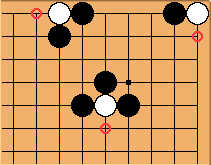
\includegraphics[width=0.47\textwidth]{atari_1}\label{fig:Gamma_0.7}}
	\hfill
	\subfloat[Example 2:The five black stones on the top right are in atari. The only liberty they have is the circled intersection.
	The group of two black stones on the lower left is also in atari. It may be captured by white (when white plays at a).]{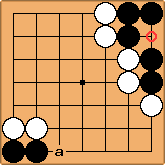
\includegraphics[width=0.43\textwidth]{atari_2}\label{fig:Karpathy}}
	\caption{Concept of Atari}
\end{figure}
\\

\subsection{Reinforcement Learning}
We present a brief overview of reinforcement learning. Reinforcement learning is an area of computer science that is designed to solve problems that have a notion of risk vs. reward. It is especially suitable for designing agents that can learn to perform actions in a given environment to maximize reward. Thus, it is well matched for solving problems such as games, which have very clear definitions of possible actions and rewards. Briefly, all reinforcement learning techniques involve learning a function $Q(s,a)$ that returns a particular reward $r$ for an action $a$ taken on a given state $s$. The agent then simply learns to take actions that maximize the cumulative reward. Reinforcement learning was given the spotlight in 1992 when Gerald Tesauro designed an agent that learned to play backgammon at a world-class skill level through self-play. However, further achievements were not possible at the time because the space of possible state-action combinations was simply too large in most other tasks for an agent to efficiently learn a good policy.

\subsection{DeepMind's Atari Agent}
The breakthrough came in 2014 when DeepMind designed an agent that could (very quickly) learn to play a variety of Atari arcade games at superhuman performance. The concept of approximating the Q-function when its true state space was too large was not new. However, DeepMind was the first to successfully train a convolutional neural network (deemed a Q-network) to approximate the Q-function. With this advancement, their agent was able to operate on the raw pixel data of the atari emulator and learn the best action.

\subsection{Testing DeepMind's approach on Go}
For us, the natural next question was whether we could make minimal modifications to DeepMind's approach, and train an agent that would learn to play Go at a decent skill level. While the state space of Go is far larger than that of the Atari games, we hypothesized that training an agent to perform to an acceptable or even poor (but better than random) level would be possible, given the advantage of explicit board representations and much smaller board sizes.
